\documentclass[../../Aurora C# unofficial manual.tex]{subfiles}

\begin{document}
	\section{Ground forces replacements}
	Original post can be found
	\href{http://aurora2.pentarch.org/index.php?topic=11593.msg140370#msg140370}{here}.
	\\\\
	
	There can be a lot of micromanagement involved in re-organising ground forces after combat, especially if you have a very detailed OOB. Therefore, I have added an automated replacement process for v1.12
	
	Each formation can be assigned a Replacement Template. By default, this is the template used to construct the formation initially. It can be changed using the 'Change Temp' button on the Order of Battle tab of the Ground Forces window. The current Replacement Template for each formation is shown on the same tab when it is selected. When you change to a different template, you have the option to change all formations with the same current template to the new template. Note the new template may have a different composition of units than the original template. You might do this to add extra capabilities or even stop replacing certain types of unit.
	
	Each formation can be assigned a replacement priority on the same tab. When replacements are available, they are assigned to formations in descending order of priority. The default priority for a new formation is 10.
	
	You can also flag a formation as 'Use for Replacements', in which case the Replacement Template is removed for that formation. During the Ground Replacement Phase, which happens in each construction phase and after ground combat, units are moved from designated replacement formations to any formations at the same population that are in need of replacements.
	\begin{figure}[H]
		\centering
		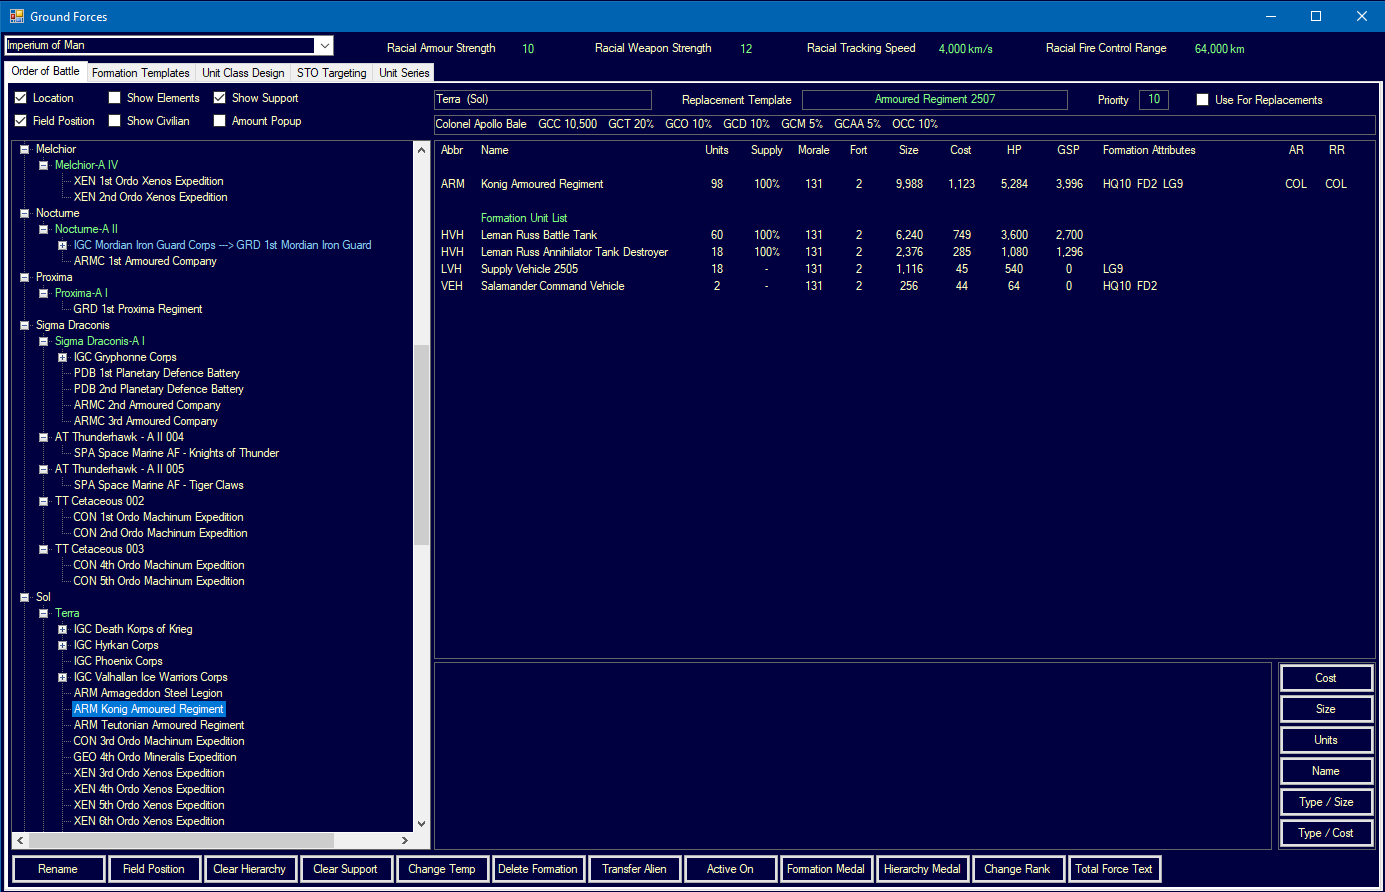
\includegraphics[width=0.95\linewidth]{images/Replacements}
		\caption[Replacements]{Ground Forces Replacements Example 1}
		\label{fig:replacements}
	\end{figure}
	
	Over time, new ground units will be designed and will often be improved versions of existing designs. For example, in my current game, I have four different versions of the Chimera, a light vehicle armed with a crew-served anti-personnel weapon. Therefore you can organise similar ground unit designs into Unit Series using a new tab for that purpose. To do so, just drag and drop from the list of non-assigned units to the desired Unit Series. Dropping on to the series name will place the unit at the top of the series. Dropping on to an existing unit in the series will place the dropped unit below the target unit. Dragging an assigned unit into empty space will remove it from a Unit Series.
	
	When replacements are required, the replacement process will use the Unit Series of each unit in the Replacement Template, rather than the actual unit. For example, assume I have a formation that was built using Chimera MK IIs and still has that same original template. When that formation looks for replacements, it will work down the Unit Series of the Chimera MK II looking for the highest unit available. In this case, the Chimera MK IV would the preferred option, followed by the MK III, etc. This means you don't have to update Replacement Templates when you create a new version of a build template with upgraded designs.
	
	This system should add a lot more flexibility and automation, while maintaining the realism aspect of shipping out replacements to the frontier. You can still use the existing drag and drop functionality for manual replacements.
	\begin{figure}[H]
		\centering
		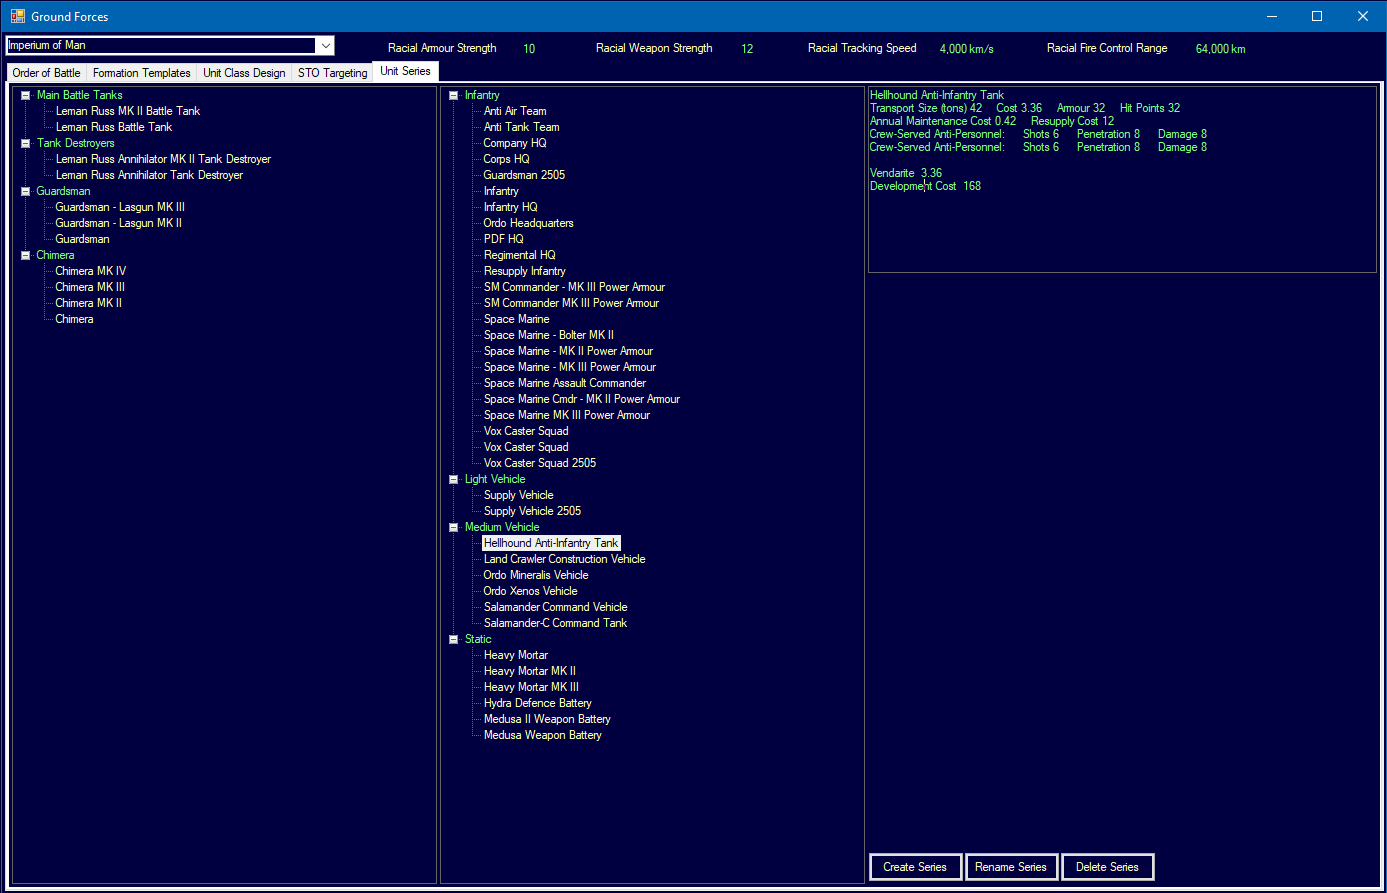
\includegraphics[width=0.95\linewidth]{images/Replacements2}
		\caption[Replacements]{Ground Forces Replacements Example 2}
		\label{fig:replacements2}
	\end{figure}
\end{document}